\documentclass[UTF8,a4paper,11pt]{ctexart}

\usepackage{amsmath,amssymb,amsthm}
\usepackage{geometry}
\usepackage{booktabs,longtable,array,multicol}
\usepackage{enumitem}
\usepackage{xcolor}
\usepackage{hyperref}
\usepackage{tikz}
\usetikzlibrary{arrows.meta,positioning,calc,shapes.geometric}

\geometry{left=1.8cm,right=1.8cm,top=2.0cm,bottom=2.0cm}
\hypersetup{colorlinks=true,linkcolor=blue!55!black,urlcolor=blue!55!black}
\setlist[itemize]{leftmargin=1.6em,itemsep=0.25em,topsep=0.25em}
\setlist[enumerate]{leftmargin=1.8em,itemsep=0.25em,topsep=0.25em}
\setlength{\parskip}{0.35em}
\setlength{\parindent}{0pt}

\newtheorem{theorem}{定理}[section]
\newtheorem{lemma}[theorem]{引理}
\newtheorem{claim}[theorem]{命题}
\newtheorem{definition}[theorem]{定义}

\newenvironment{algobox}[1]
{\par\medskip\noindent\begin{minipage}{0.96\linewidth}\hrule\vspace{0.35em}\textbf{#1}\par\vspace{0.25em}\small}
{\par\vspace{0.25em}\hrule\end{minipage}\par\medskip}

\newcommand{\Time}{\mathrm{Time}}
\newcommand{\OPT}{\mathrm{OPT}}
\newcommand{\poly}{\mathrm{poly}}
\newcommand{\NP}{\mathsf{NP}}
\newcommand{\Pclass}{\mathsf{P}}
\newcommand{\NPC}{\mathsf{NP\mbox{-}complete}}
\newcommand{\NPH}{\mathsf{NP\mbox{-}hard}}

\title{\textbf{CS216 Algorithm Design and Analysis (H)\\期末复习 Notes}}
\author{Yanqiao Chen \\ 
       Southern University of Science and Technology\\
       \texttt{12412115@mail.sustech.edu.cn}}
\date{2026 年 6 月}

\begin{document}
\maketitle
\tableofcontents
\newpage

\section{考试结构与使用路线}

期末题型可按如下方式准备：前半部分是 $10$ 道不定项选择题，考定义、条件、复杂度和经典反例；后半部分是 $6$ 道大题，通常一章一道，覆盖
\[
\text{Greedy},\quad
\text{Divide and Conquer},\quad
\text{Dynamic Programming},\quad
\text{Reduction},\quad
\text{Network Flow},\quad
\text{Randomized Algorithms}.
\]
大题不是背原题，而是把新叙述翻译成课程模型，再写算法、正确性证明和复杂度。

\subsection{大题固定答题模板}

每道设计题建议写成五段：
\begin{enumerate}
  \item \textbf{Model.} 说明题目等价于哪个经典模型，或为什么可以用某个算法范式。
  \item \textbf{Algorithm.} 写清输入预处理、核心步骤、输出规则，最好给伪代码。
  \item \textbf{Correctness.} 贪心写 exchange/stays-ahead；DP 写归纳；流写 cut/closure 等价；归约写 iff；随机写期望或概率界。
  \item \textbf{Complexity.} 给出排序、建图、DP 表规模、流算法调用等主导项。
  \item \textbf{Edge cases.} 说明不可行、负权、容量下界、强制不选、空解等特殊情况。
\end{enumerate}

\subsection{选择题高频清单}

\begin{multicols}{2}
\begin{itemize}
  \item $O,\Omega,\Theta$ 的定义与方向。
  \item Efficient = worst-case polynomial time。
  \item Gale-Shapley: $O(n^2)$，proposer-optimal。
  \item Interval scheduling 选最早结束。
  \item Interval partitioning 最少教室数 = depth。
  \item Dijkstra 要非负边权。
  \item Huffman 每次合并最低频率。
  \item Ford-Fulkerson 使用 residual network。
  \item Max-flow min-cut theorem。
  \item Integrality theorem。
  \item NP-complete 证明三步。
  \item Monte Carlo 与 Las Vegas 的区别。
  \item Union bound: $\Pr[\cup_i A_i]\le \sum_i\Pr[A_i]$。
  \item Chernoff bound 的指数衰减形态。
\end{itemize}
\end{multicols}

\newpage
\section{Algorithm Analysis}

\subsection{多项式时间、输入规模与渐近记号}

课程中的 tractability 采用工作定义：一个算法若在最坏情况下运行时间为输入规模 $n$ 的多项式，即存在常数 $a,b>0$ 使
\[
T(n)\le a n^b,
\]
则称为 efficient algorithm。注意这只是理论上的可处理性定义：某些多项式算法常数巨大，某些指数算法在小规模或特殊分布上仍实用。

\begin{definition}[渐近上界、下界与紧界]
\[
T(n)=O(f(n)) \iff \exists c>0,n_0,\ \forall n\ge n_0,\ 0\le T(n)\le c f(n).
\]
\[
T(n)=\Omega(f(n)) \iff \exists c>0,n_0,\ \forall n\ge n_0,\ T(n)\ge c f(n)\ge 0.
\]
\[
T(n)=\Theta(f(n)) \iff T(n)=O(f(n)) \text{ and } T(n)=\Omega(f(n)).
\]
\end{definition}

常见增长顺序：
\[
\log n \ll n \ll n\log n \ll n^2 \ll n^3 \ll n^k \ll c^n \ll n!.
\]
常用关系：
\[
\log_a n=\Theta(\log_b n),\qquad \log^a n=O(n^c),\qquad n^c=O(r^n)\ (r>1),
\]
\[
n! = 2^{\Theta(n\log n)}.
\]

\subsection{代表问题光谱}

课件用 independent set 串起从易到难的问题：
\begin{center}
\begin{tabular}{lll}
\toprule
问题 & 典型方法 & 复杂度/难度\\
\midrule
Interval Scheduling & Greedy & $O(n\log n)$\\
Weighted Interval Scheduling & DP & $O(n\log n)$\\
Bipartite Matching & Network Flow & polynomial\\
Independent Set & Reduction/NP-complete & NP-complete\\
Competitive Facility Location & Game/PSPACE & 更难\\
\bottomrule
\end{tabular}
\end{center}

选择题易错点：``comparison sorting 至少需要 $O(n\log n)$ 次比较''不是严格说法；下界应写作 $\Omega(n\log n)$。

\section{Stable Matching}

\subsection{定义}

一对一稳定匹配中，给定 $n$ 个 men 与 $n$ 个 women，每个人有严格偏好表。
\begin{itemize}
  \item \textbf{Perfect matching:} 每个人恰好匹配一个对象。
  \item \textbf{Unstable/blocking pair:} 未匹配的一对 $(m,w)$ 彼此都更喜欢对方胜过当前 partner。
  \item \textbf{Stable matching:} perfect matching 且不存在 blocking pair。
\end{itemize}
普通 roommate problem 不是二分结构，稳定匹配不一定存在；marriage problem 中稳定匹配总存在。

\subsection{Gale-Shapley 算法}

\begin{algobox}{Gale-Shapley, men-proposing version}
\begin{enumerate}
  \item 初始所有 men 与 women 都 free。
  \item 当存在 free man $m$ 且 $m$ 尚未向所有 woman proposal：
  \begin{enumerate}
    \item $m$ 向自己偏好表中尚未 proposal 的最高-ranked woman $w$ 求婚。
    \item 若 $w$ free，则暂时匹配 $(m,w)$。
    \item 若 $w$ 当前匹配 $m'$ 且 $w$ 更喜欢 $m$，则改匹配 $(m,w)$，并令 $m'$ free。
    \item 否则 $w$ 拒绝 $m$。
  \end{enumerate}
  \item 输出所有暂时匹配。
\end{enumerate}
\end{algobox}

\begin{center}
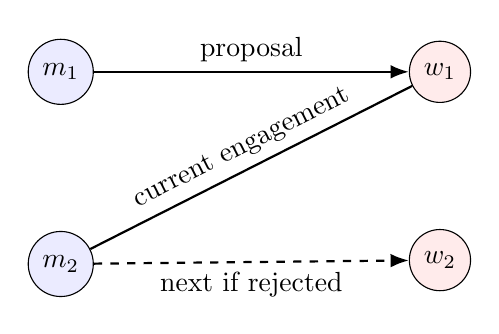
\begin{tikzpicture}[node distance=1.6cm,>=Latex]
  \node[circle,draw,fill=blue!8] (m1) {$m_1$};
  \node[circle,draw,fill=blue!8,below=of m1] (m2) {$m_2$};
  \node[circle,draw,fill=red!8,right=4cm of m1] (w1) {$w_1$};
  \node[circle,draw,fill=red!8,below=of w1] (w2) {$w_2$};
  \draw[->,thick] (m1) -- node[above] {proposal} (w1);
  \draw[->,thick,dashed] (m2) -- node[below] {next if rejected} (w2);
  \draw[thick] (m2) -- node[above,sloped] {current engagement} (w1);
\end{tikzpicture}
\end{center}

\subsection{正确性证明}

\begin{lemma}[终止性]
算法最多进行 $n^2$ 次 proposal。
\end{lemma}
\begin{proof}
每次循环产生一个之前没有发生过的 ordered pair proposal $(m,w)$。共有 $n^2$ 对，因此循环次数至多 $n^2$。
\end{proof}

\begin{lemma}[完美性]
算法终止时所有人都被匹配。
\end{lemma}
\begin{proof}
一旦某个 woman 收到 proposal，她之后始终保持 matched：她只会把当前 partner 换成更喜欢的人，不会变成 unmatched。若终止时某个 man $m$ unmatched，则由于循环已停，$m$ 必然已向所有 women proposal。于是所有 women 都至少收到过 proposal，从而全都 matched。此时有 $n$ 个 women matched，意味着 $n$ 个 men matched，与 $m$ unmatched 矛盾。
\end{proof}

\begin{theorem}[稳定性]
Gale-Shapley 输出稳定匹配。
\end{theorem}
\begin{proof}
设输出为 $S$。若存在 blocking pair $(m,w)$，即 $m$ 更喜欢 $w$ 胜过 $S(m)$，且 $w$ 更喜欢 $m$ 胜过 $S(w)$。因为 $m$ 按偏好从高到低 proposal，$m$ 在向 $S(m)$ proposal 前一定已向 $w$ proposal。考虑当时 $w$ 的反应：
\begin{itemize}
  \item 若 $w$ 拒绝 $m$，说明当时 $w$ 已有更喜欢的 partner。之后 $w$ 只会 trade up，所以最终 $S(w)$ 仍比 $m$ 好。
  \item 若 $w$ 接受 $m$，但最终没和 $m$ 匹配，说明后来 $w$ 抛弃 $m$ 换到更喜欢的人，最终 $S(w)$ 仍比 $m$ 好。
\end{itemize}
两种情况都与 $w$ 更喜欢 $m$ 矛盾，因此不存在 blocking pair。
\end{proof}

\subsection{最优性与一对多版本}

Men-proposing GS 输出 \textbf{man-optimal} stable matching，同时是 \textbf{woman-pessimal} stable matching。直觉上，每个 man 都按自己的偏好从高到低尝试；一旦被某个 woman 永久拒绝，他不可能在任何稳定匹配中得到她，否则会构成阻塞对。

Hospitals/Residents 是 one-to-many 版本：医院有 capacity，学生向医院申请，医院始终保留最喜欢的若干学生并拒绝其余学生。扩展 GS 仍能求稳定匹配。Rural Hospital Theorem: 某些医院在所有稳定匹配中得到相同数量，甚至相同集合的学生。

\begin{algobox}{Extended Gale-Shapley for Hospitals/Residents}
\begin{enumerate}
  \item 对每个 student $s$，按偏好维护尚未申请的 hospital 列表；每个 hospital $h$ 有容量 $q_h$。
  \item 初始化所有 students 为 free，每个 hospital 的暂录集合 $A_h=\emptyset$。
  \item 当存在 free student $s$ 且 $s$ 还有可申请 hospital：
  \begin{enumerate}
    \item $s$ 向列表中最高偏好且未申请过的 $h$ 申请。
    \item 将 $s$ 临时加入 $A_h$。
    \item 若 $|A_h|>q_h$，从 $A_h$ 中删去 $h$ 最不喜欢的 student $s'$，令 $s'$ free。
  \end{enumerate}
  \item 输出所有 $A_h$。
\end{enumerate}
复杂度：若共有 $L$ 对 acceptable pairs，用堆维护每个 hospital 的最差暂录者，则申请阶段为 $O(L\log q_{\max})$。
\end{algobox}

\section{Greedy Algorithms}

\subsection{证明模板}

贪心大题最重要的不是算法本身，而是证明所选局部动作不会伤害全局最优性。常见模板：
\begin{itemize}
  \item \textbf{Stays ahead:} 证明贪心解第 $i$ 步之后至少不差于任意最优解第 $i$ 步。
  \item \textbf{Exchange argument:} 取一个与贪心前缀最长相同的最优解，把它下一步替换成贪心选择，证明可行且目标值不变差。
  \item \textbf{Structural lower bound:} 先证明任何解都至少需要某个数量，再证明贪心达到该数量。
  \item \textbf{Safe choice + induction:} 证明存在一个最优解包含贪心选择，再递归处理剩余实例。
\end{itemize}

\subsection{Selecting Breakpoints}

油箱容量为 $c$，沿路加油站位置为 $b_1<\cdots<b_n$，目标是最少停车。贪心：每次从当前位置开到可达范围内最远的加油站。

\begin{theorem}
最远可达加油贪心是最优的。
\end{theorem}
\begin{proof}
设贪心停靠序列为 $g_0,g_1,\ldots$，某个最优解为 $f_0,f_1,\ldots$。取与贪心前缀相同最长的最优解，即 $f_i=g_i$ 对 $i\le r$。由于 $g_{r+1}$ 是从 $g_r$ 出发可达的最远站点，而 $f_{r+1}$ 也必须从 $g_r$ 可达，所以 $g_{r+1}\ge f_{r+1}$。把最优解中的 $f_{r+1}$ 换成 $g_{r+1}$ 不会增加停靠次数，也不会破坏后续可行性，因为站点更靠后只会让后面距离更短。于是得到一个与贪心有更长公共前缀的最优解，矛盾。
\end{proof}

\subsection{Interval Scheduling}

问题：给定区间 $[s_j,f_j)$，选最多数量互不重叠区间。贪心按结束时间递增排序，每次选择与已选区间兼容且结束最早的区间。

\begin{algobox}{Interval-Scheduling}
\begin{enumerate}
  \item 按 $f_j$ 从小到大排序。
  \item 令 $A=\emptyset$，$t=-\infty$。
  \item 依次扫描区间 $j$：若 $s_j\ge t$，则选择 $j$ 并令 $t=f_j$。
  \item 返回 $A$。
\end{enumerate}
\end{algobox}

\begin{center}
\begin{tikzpicture}[x=0.75cm,y=0.65cm]
  \draw[->] (0,0) -- (10,0) node[right] {time};
  \foreach \x in {1,...,9} \draw (\x,0.08)--(\x,-0.08);
  \draw[line width=2pt,blue] (0.8,1) -- (3.0,1) node[right] {$a$};
  \draw[line width=2pt,red] (1.5,2) -- (4.5,2) node[right] {$b$};
  \draw[line width=2pt,blue] (3.2,1) -- (5.0,1) node[right] {$c$};
  \draw[line width=2pt,red] (4.0,3) -- (7.2,3) node[right] {$d$};
  \draw[line width=2pt,blue] (5.4,1) -- (8.0,1) node[right] {$e$};
  \node[blue] at (4.7,-0.65) {选结束最早的兼容区间，蓝色为一种贪心结果};
\end{tikzpicture}
\end{center}

\begin{theorem}
按最早结束时间选择的算法最优。
\end{theorem}
\begin{proof}
设贪心选择 $i_1,i_2,\ldots,i_k$，任意最优解选择 $j_1,j_2,\ldots,j_m$，均按结束时间排序。证明 $f_{i_r}\le f_{j_r}$ 对所有 $r\le \min(k,m)$ 成立。$r=1$ 时贪心选全局结束最早区间，成立。若 $f_{i_{r-1}}\le f_{j_{r-1}}$，则 $j_r$ 与 $j_{r-1}$ 兼容，所以 $s_{j_r}\ge f_{j_{r-1}}\ge f_{i_{r-1}}$，即 $j_r$ 在贪心第 $r$ 步也是候选区间。贪心选结束最早候选，因此 $f_{i_r}\le f_{j_r}$。若 $m>k$，则 $j_{k+1}$ 在贪心选完 $i_k$ 后仍兼容，贪心不应停止，矛盾。故 $k=m$。
\end{proof}

\subsection{Interval Partitioning}

问题：用最少教室安排所有 lectures。贪心按开始时间排序，把每个 lecture 放入当前结束最早且可用的教室；若无可用教室，则开新教室。最少教室数等于 intervals 的 \textbf{depth}，即某个时刻同时重叠的最大区间数。

正确性：若贪心开第 $d$ 间教室，说明当前 lecture 开始时已有 $d-1$ 间教室都被未结束 lecture 占用，因此存在 $d$ 个区间在当前开始时刻重叠，depth 至少为 $d$。任何方案至少需要 depth 间教室，而贪心用了 $d$ 间，所以最优。

\subsection{Minimizing Maximum Lateness}

每个 job 有处理时间 $t_j$ 与 deadline $d_j$，无释放时间，目标最小化
\[
L_{\max}=\max_j(C_j-d_j).
\]
Earliest Deadline First (EDF) 按 $d_j$ 递增处理。

证明用 exchange argument。若某个最优 schedule 中存在相邻 inversion：$d_i>d_j$ 但 $i$ 在 $j$ 前。交换 $i,j$ 后，其它 job completion time 不变；$j$ 更早完成，lateness 不增；$i$ 的新 completion time 等于原来 $j$ 的 completion time，且 $d_i>d_j$，所以 $i$ 的 lateness 不超过原来 $j$ 的 lateness。因此交换不会增大 $L_{\max}$。不断消除 inversion 得到 EDF，故 EDF 最优。

\subsection{Caching: Farthest-in-Future}

Offline caching 已知完整请求序列，cache 容量为 $k$。Belady/Farthest-in-Future: cache miss 且需驱逐时，驱逐下一次使用时间最晚的 item，若不再使用则优先驱逐。

证明思路：对任意最优 schedule $S$，按时间归纳把它改造成与 FF 前 $j$ 步行为一致且不增加 miss 数的最优 schedule。第 $j+1$ 步若不驱逐或驱逐同一 item，显然成立；若驱逐不同 item，用 FF 驱逐的 item 替换 $S$ 驱逐的 item。因为 FF 被驱逐 item 的下一次请求不早于 $S$ 驱逐 item 的下一次请求，这种替换不会在更早时刻造成额外 miss。

\subsection{Dijkstra, MST, Huffman, Directed MST}

\textbf{Dijkstra.} 在非负边权图中维护已确定集合 $S$，每次取 $V-S$ 中估计距离最小的点 $v$ 加入 $S$ 并 relax 出边。正确性关键：非负边保证任何从 $s$ 到未确定点再回到 $v$ 的路径不会比当前 $d(v)$ 更短。

\begin{algobox}{Dijkstra$(G,s)$}
\begin{enumerate}
  \item 对所有 $v$，令 $d[v]=\infty$；令 $d[s]=0$。把所有点放入按 $d$ 排序的 priority queue。
  \item 当队列非空：
  \begin{enumerate}
    \item 取出 $d$ 最小的未确定点 $u$。
    \item 对每条边 $(u,v)$，若 $d[v]>d[u]+w(u,v)$，则更新 $d[v]$ 并 decrease-key。
  \end{enumerate}
  \item 返回所有 $d[v]$。
\end{enumerate}
二叉堆实现为 $O((m+n)\log n)$；边权必须非负。
\end{algobox}

\textbf{MST.} Cut property: 对任意 cut，跨越该 cut 的最轻边属于某棵 MST。Cycle property: 一个环上最重边不必属于 MST。Kruskal 按边权递增加不成环的边；Prim 每次从当前树跨 cut 取最轻边。

\begin{algobox}{Kruskal$(G)$}
\begin{enumerate}
  \item 将所有边按权重从小到大排序，初始化并查集，每个点单独成分。
  \item 令 $T=\emptyset$。
  \item 依次扫描边 $e=(u,v)$：
  \begin{enumerate}
    \item 若 $\mathrm{find}(u)\ne \mathrm{find}(v)$，则把 $e$ 加入 $T$ 并 union 两个连通块。
    \item 否则跳过 $e$，因为加入会成环。
  \end{enumerate}
  \item 返回 $T$。
\end{enumerate}
复杂度 $O(m\log m)$，正确性来自 cut property。
\end{algobox}

\textbf{Huffman.} 每次合并频率最低的两个符号。正确性用 safe choice：在某棵最优前缀码树中，最低频的两个字符可以作为最深层 siblings；合并为伪字符后递归求最优。

\begin{algobox}{Huffman-Coding}
\begin{enumerate}
  \item 为每个字符 $a$ 建叶子节点，key 为频率 $f_a$，放入 min-priority queue。
  \item 当队列中节点数大于 $1$：
  \begin{enumerate}
    \item 取出频率最小的两个节点 $x,y$。
    \item 新建父节点 $z$，令 $f_z=f_x+f_y$，左右孩子为 $x,y$。
    \item 将 $z$ 插回队列。
  \end{enumerate}
  \item 队列中唯一节点即最优前缀码树根。
\end{enumerate}
复杂度 $O(n\log n)$。
\end{algobox}

\textbf{Chu-Liu/Edmonds Directed MST.} 对固定 root 的最小入枝树：每个非 root 点先选最小入边；若无环则完成；若有有向环，缩成一个超级点，并对进入环的边 $(u,v)$ 调整权重为 $w(u,v)-w(\mathrm{in}(v))$，递归求解后展开。调整权重表示进入环时需要替换掉 $v$ 的原最小入边。

\begin{algobox}{Chu-Liu/Edmonds$(G,r)$}
\begin{enumerate}
  \item 对每个 $v\ne r$，选入边中权重最小的一条 $\mathrm{in}[v]$；若某点无入边，则不存在入枝树。
  \item 若这些边不含有向环，返回它们。
  \item 若存在有向环 $C$：
  \begin{enumerate}
    \item 将 $C$ 缩成超级点 $c$。
    \item 对每条从环外进入环内点 $v\in C$ 的边 $(u,v)$，新权重设为 $w(u,v)-w(\mathrm{in}[v])$。
    \item 在缩点图上递归求最小入枝树。
    \item 展开 $C$：若递归解选择进入 $C$ 的边对应原边 $(u,v)$，则保留环上所有 $\mathrm{in}[\cdot]$，但删除 $\mathrm{in}[v]$。
  \end{enumerate}
\end{enumerate}
朴素实现 $O(nm)$；高级堆优化可更快。
\end{algobox}

\subsection{Exam Greedy: 交易时间匹配}

题型：旧账户交易时间 $t_j$ 带容差 $e_j$，新账户交易时间 $m_i$；若 $|m_i-t_j|\le e_j$ 可匹配，一笔交易只能用一次，判断是否能全部匹配。

可以建二分图并跑最大匹配，$O(n^3)$ 也通常能接受；若要求 $O(n^2)$，可用区间贪心：旧交易 $j$ 对应新交易可落入区间 $[t_j-e_j,t_j+e_j]$。按新交易时间排序；扫描 $m_i$，把所有左端点 $\le m_i$ 的旧交易加入以右端点为 key 的小根堆；删除右端点 $<m_i$ 的过期区间；若堆空则失败，否则把右端点最小的区间匹配给 $m_i$。

正确性：这是 earliest deadline first。若某一步新交易 $m_i$ 可匹配多个旧交易，选择右端点最小者最安全；任何可行解若把 $m_i$ 给了更晚截止的区间 $B$，而最早截止区间 $A$ 给了之后某个 $m_{i'}\ge m_i$，则交换后 $A$ 仍能匹配 $m_i$，$B$ 仍能匹配 $m_{i'}$，可行性不变。

\section{Divide and Conquer}

\subsection{Master Theorem}

对于
\[
T(n)=aT(n/b)+O(n^d),\qquad a\ge 1,\ b>1,
\]
比较 $a$ 与 $b^d$：
\[
T(n)=
\begin{cases}
O(n^d), & a<b^d,\\
O(n^d\log n), & a=b^d,\\
O(n^{\log_b a}), & a>b^d.
\end{cases}
\]
直觉：递归树第 $\ell$ 层有 $a^\ell$ 个子问题，每个规模 $n/b^\ell$，该层代价为
\[
a^\ell\left(\frac{n}{b^\ell}\right)^d=n^d\left(\frac{a}{b^d}\right)^\ell.
\]

\subsection{Counting Inversions}

inversion 是 $i<j$ 且 $a_i>a_j$。分治类似 merge sort：递归统计左半、右半 inversion，merge 时统计 cross inversion。当左指针元素 $L[i]>R[j]$，由于 $L[i],L[i+1],\ldots$ 均大于 $R[j]$，增加 $|L|-i+1$ 个 inversion。复杂度
\[
T(n)=2T(n/2)+O(n)=O(n\log n).
\]

\begin{algobox}{Sort-and-Count$(A)$}
\begin{enumerate}
  \item 若 $|A|\le 1$，返回 $(A,0)$。
  \item 将 $A$ 分为左右两半，递归得到 $(L,c_L)$ 与 $(R,c_R)$。
  \item Merge $L,R$：
  \begin{enumerate}
    \item 若 $L[i]\le R[j]$，输出 $L[i]$，$i\leftarrow i+1$。
    \item 若 $L[i]>R[j]$，输出 $R[j]$，并令 $c_M\leftarrow c_M+(|L|-i+1)$，$j\leftarrow j+1$。
  \end{enumerate}
  \item 返回合并后有序数组与 $c_L+c_R+c_M$。
\end{enumerate}
\end{algobox}

\subsection{Closest Pair}

平面最近点对：
\begin{enumerate}
  \item 按 $x$ 排序分成左右两半，递归求 $\delta_L,\delta_R$，令 $\delta=\min(\delta_L,\delta_R)$。
  \item 只需检查中线两侧距离 $<\delta$ 的 strip。
  \item strip 中按 $y$ 排序，每个点只需检查后面常数个点。
\end{enumerate}
正确性关键：若最优点对跨越分割线且距离 $<\delta$，两点必在 strip 内；packing argument 说明在 $\delta\times 2\delta$ 邻域内候选点数为常数。若每层维护按 $y$ 排序列表，可达 $O(n\log n)$。

\subsection{Integer Multiplication, Karatsuba, Matrix Multiplication}

普通分治乘法把 $x=x_1 10^m+x_0$，$y=y_1 10^m+y_0$，需四次子乘法：
\[
xy=x_1y_1 10^{2m}+(x_1y_0+x_0y_1)10^m+x_0y_0.
\]
Karatsuba 用三次子乘法：
\[
p=x_1y_1,\quad q=x_0y_0,\quad r=(x_1+x_0)(y_1+y_0),
\]
\[
xy=p10^{2m}+(r-p-q)10^m+q,
\]
因此
\[
T(n)=3T(n/2)+O(n)=O(n^{\log_2 3}).
\]
Strassen 矩阵乘法用 $7$ 次半规模矩阵乘法代替 $8$ 次，复杂度 $O(n^{\log_2 7})$。

\subsection{FFT 与卷积}

多项式乘法可转成三步：
\[
\text{coefficients}\xrightarrow{\mathrm{FFT}}\text{values}
\xrightarrow{\text{pointwise multiply}}\text{values}
\xrightarrow{\mathrm{IFFT}}\text{coefficients}.
\]
若 $A(x),B(x)$ 次数小于 $n$，取 $N\ge 2n$ 的单位根 $\omega_N=e^{2\pi i/N}$。DFT:
\[
\hat A_k=A(\omega_N^k),\quad k=0,\ldots,N-1.
\]
Cooley-Tukey 分解：
\[
A(x)=A_{\mathrm{even}}(x^2)+xA_{\mathrm{odd}}(x^2),
\]
\[
A(\omega_N^k)=A_e(\omega_{N/2}^k)+\omega_N^k A_o(\omega_{N/2}^k),
\]
\[
A(\omega_N^{k+N/2})=A_e(\omega_{N/2}^k)-\omega_N^k A_o(\omega_{N/2}^k).
\]
复杂度 $T(N)=2T(N/2)+O(N)=O(N\log N)$。

\begin{algobox}{Recursive-FFT$(a,\omega)$}
\begin{enumerate}
  \item 若 $n=1$，返回 $a$。
  \item 令 $a^{(0)}=(a_0,a_2,\ldots,a_{n-2})$，$a^{(1)}=(a_1,a_3,\ldots,a_{n-1})$。
  \item $y^{(0)}=\mathrm{FFT}(a^{(0)},\omega^2)$，$y^{(1)}=\mathrm{FFT}(a^{(1)},\omega^2)$。
  \item 对 $k=0,\ldots,n/2-1$：
  \[
  y_k=y^{(0)}_k+\omega^k y^{(1)}_k,\qquad
  y_{k+n/2}=y^{(0)}_k-\omega^k y^{(1)}_k.
  \]
  \item 返回 $y$。
\end{enumerate}
IFFT 使用 $\omega^{-1}$ 再整体除以 $n$。
\end{algobox}

\begin{center}
\begin{tikzpicture}[>=Latex,node distance=1.3cm]
  \node[draw,rounded corners] (a) {系数 $A,B$};
  \node[draw,rounded corners,right=of a] (b) {FFT 求值};
  \node[draw,rounded corners,right=of b] (c) {逐点相乘};
  \node[draw,rounded corners,right=of c] (d) {IFFT 插值};
  \node[draw,rounded corners,right=of d] (e) {卷积系数};
  \draw[->] (a)--(b);
  \draw[->] (b)--(c);
  \draw[->] (c)--(d);
  \draw[->] (d)--(e);
\end{tikzpicture}
\end{center}

\subsection{Exam D\&C: 完全二叉树局部最小}

题型：完全二叉树中，一个点若不大于所有邻居（父亲和孩子）则为 local minimum。从 root 出发，只访问到节点才知道值，要求 $O(\log n)$。

\begin{algobox}{Find-Local-Minimum}
\begin{enumerate}
  \item 从根 $v$ 开始。
  \item 若 $v$ 不大于所有存在的邻居，返回 $v$。
  \item 否则移动到一个值严格小于 $v$ 的邻居。为了保证向下 $O(\log n)$，若某个孩子更小，就移动到更小的孩子；根开始无需向父亲移动。
  \item 重复直到返回或到叶子。
\end{enumerate}
\end{algobox}

\begin{center}
\begin{tikzpicture}[level distance=1.0cm,sibling distance=2.2cm,
  every node/.style={circle,draw,minimum size=0.75cm}]
  \node[fill=red!10] {9}
    child { node[fill=yellow!20] {5}
      child { node[fill=green!20] {3} }
      child { node {7} } }
    child { node {11}
      child { node {12} }
      child { node {13} } };
  \node[draw=none,rectangle,below=3.3cm] {沿严格下降边走，值序列单调下降，叶深为 $O(\log n)$};
\end{tikzpicture}
\end{center}

正确性：每次若当前点不是 local minimum，则存在邻居更小。沿更小孩子向下走，值严格下降，不会成环；若最终到达叶子，叶子没有孩子且其值小于父亲，因此是 local minimum。若中途停下，则按条件已经不大于所有邻居。完全二叉树高度为 $O(\log n)$，所以访问 $O(\log n)$ 个节点。

\section{Dynamic Programming}

\subsection{DP 答题模板}

DP 大题必须写清四件事：
\[
\text{state} \rightarrow \text{transition} \rightarrow \text{order/base cases} \rightarrow \text{answer/complexity}.
\]
正确性通常用归纳：假设所有更小子问题最优，转移枚举了最后一步或关键选择，因此得到当前子问题最优。

\subsection{Weighted Interval Scheduling}

区间 $j$ 有权重 $v_j$，按结束时间排序。令
\[
p(j)=\max\{i<j:f_i\le s_j\}
\]
为与 $j$ 兼容的最后区间。状态 $M[j]$ 表示只考虑前 $j$ 个区间的最大权重：
\[
M[j]=\max\{M[j-1],\ v_j+M[p(j)]\},\qquad M[0]=0.
\]
若不选 $j$，答案为 $M[j-1]$；若选 $j$，之前只能来自 $p(j)$。二分预处理 $p(j)$ 后复杂度 $O(n\log n)$，DP 本身 $O(n)$。

\begin{algobox}{Weighted-Interval-Scheduling}
\begin{enumerate}
  \item 按结束时间排序区间，使 $f_1\le\cdots\le f_n$。
  \item 对每个 $j$，二分求 $p(j)=\max\{i<j:f_i\le s_j\}$。
  \item 令 $M[0]=0$。
  \item 对 $j=1,\ldots,n$：
  \[
  M[j]=\max\{M[j-1],\ v_j+M[p(j)]\}.
  \]
  \item 若需恢复解，从 $j=n$ 倒推：若 $v_j+M[p(j)]>M[j-1]$，选 $j$ 并跳到 $p(j)$；否则跳到 $j-1$。
\end{enumerate}
\end{algobox}

\subsection{Segmented Least Squares}

给定点 $(x_i,y_i)$，用若干线段拟合，目标为误差加每段固定成本 $C$。预处理每个区间 $[i,j]$ 的最小平方误差 $e(i,j)$。状态 $M[j]$ 表示拟合前 $j$ 个点的最小代价：
\[
M[j]=\min_{1\le i\le j}\{M[i-1]+e(i,j)+C\},\qquad M[0]=0.
\]
正确性：最优解的最后一段必然覆盖某个后缀 $i,\ldots,j$，枚举该 $i$ 即覆盖所有可能。

\subsection{Knapsack}

0/1 背包：item $i$ 重量 $w_i$，价值 $v_i$，容量 $W$。状态 $M[i,w]$ 表示前 $i$ 个 item、容量 $w$ 的最大价值：
\[
M[i,w]=
\begin{cases}
M[i-1,w], & w_i>w,\\
\max\{M[i-1,w],\ M[i-1,w-w_i]+v_i\}, & w_i\le w.
\end{cases}
\]
时间 $O(nW)$，这是 pseudo-polynomial，不是关于输入 bit-length 的强多项式。

\begin{algobox}{0/1-Knapsack}
\begin{enumerate}
  \item 初始化 $M[0,w]=0$，对所有 $0\le w\le W$。
  \item 对 $i=1,\ldots,n$：
  \begin{enumerate}
    \item 对 $w=0,\ldots,W$：
    \[
    M[i,w]=
    \begin{cases}
    M[i-1,w], & w_i>w,\\
    \max\{M[i-1,w],M[i-1,w-w_i]+v_i\}, & w_i\le w.
    \end{cases}
    \]
  \end{enumerate}
  \item 返回 $M[n,W]$。
\end{enumerate}
滚动数组优化时，$w$ 必须从 $W$ 递减到 $w_i$，防止同一物品被重复使用。
\end{algobox}

\subsection{RNA Secondary Structure}

区间 DP。令 $OPT[i,j]$ 为子串 $i,\ldots,j$ 的最大配对数。若 $j$ 不配对，则 $OPT[i,j-1]$；若 $j$ 与 $t$ 配对，需要满足碱基互补和间隔约束，然后左右分裂：
\[
OPT[i,j]=\max\left\{OPT[i,j-1],\ \max_t\left(1+OPT[i,t-1]+OPT[t+1,j-1]\right)\right\}.
\]
按区间长度递增计算。

\subsection{Sequence Alignment 与 Hirschberg}

序列比对状态 $OPT[i,j]$ 表示 $x_1\ldots x_i$ 与 $y_1\ldots y_j$ 的最小代价：
\[
OPT[i,j]=\min\begin{cases}
OPT[i-1,j-1]+\alpha_{x_i,y_j},\\
OPT[i-1,j]+\delta,\\
OPT[i,j-1]+\delta.
\end{cases}
\]
普通 DP 时间 $O(mn)$、空间 $O(mn)$。若只要代价，可滚动数组降到 $O(n)$；若要恢复路径，Hirschberg 用分治加正向/反向 DP 找中点，空间 $O(n)$。

\subsection{Shortest Paths with Negative Edges}

Bellman-Ford DP 形式：令 $M[i,v]$ 为从 $s$ 到 $v$ 使用至多 $i$ 条边的最短路：
\[
M[i,v]=\min\left(M[i-1,v],\min_{(u,v)\in E}\{M[i-1,u]+w(u,v)\}\right).
\]
无负环时，最短简单路最多 $n-1$ 条边，所以计算到 $i=n-1$。若第 $n$ 轮仍能 relax，则存在从 $s$ 可达的负环。

\begin{algobox}{Bellman-Ford$(G,s)$}
\begin{enumerate}
  \item 初始化 $d[s]=0$，$d[v]=\infty$ for $v\ne s$。
  \item 重复 $n-1$ 轮：
  \begin{enumerate}
    \item 对每条边 $(u,v)$，若 $d[v]>d[u]+w(u,v)$，则更新 $d[v]$。
  \end{enumerate}
  \item 再扫描所有边：若仍可 relax，则报告存在从 $s$ 可达的负环。
  \item 否则返回所有 $d[v]$。
\end{enumerate}
复杂度 $O(nm)$。
\end{algobox}

\subsection{Exam DP: 库存/仓储}

题型：每月初可花固定价格 $P$ 进货任意数量；每月卖出 $c_i$ 台；仓库容量 $W$；每月底每台库存付 $F$；求最小购买与存储成本。

令 $dp[i][j]$ 表示第 $i$ 个月结束后库存为 $j$，满足前 $i$ 个月需求的最小成本。转移可枚举上月库存 $k$ 与是否购买。月初拥有 $k$，若不买则必须 $k\ge c_i$，月底 $j=k-c_i$；若购买一次，购买数量任意，固定成本 $P$，只需能使月底为 $j$，即买入 $c_i+j-k>0$。
\[
dp[i][j]=Fj+\min\left(
\min_{\substack{0\le k\le W\\k=c_i+j}} dp[i-1][k],\
P+\min_{\substack{0\le k\le W\\k<c_i+j}} dp[i-1][k]
\right).
\]
边界 $dp[0][0]=0$，$dp[0][j>0]=\infty$。答案 $\min_j dp[n][j]$，时间 $O(nW^2)$，可用前缀最小值优化到 $O(nW)$。正确性由最后一个月结束库存 $j$ 与上月库存 $k$ 的完整枚举得到。

\section{Network Flow}

\subsection{基本定义}

流网络 $G=(V,E)$ 有源点 $s$、汇点 $t$、容量 $c_e\ge 0$。流 $f$ 满足：
\[
0\le f(e)\le c_e,
\]
对所有 $v\ne s,t$，
\[
\sum_{e\text{ into }v}f(e)=\sum_{e\text{ out of }v}f(e).
\]
流值
\[
|f|=\sum_{(s,v)}f(s,v)-\sum_{(v,s)}f(v,s).
\]
$s$-$t$ cut 是划分 $(A,B)$，其中 $s\in A,t\in B$；cut capacity:
\[
c(A,B)=\sum_{u\in A,v\in B}c(u,v).
\]

\subsection{Residual Network 与 Ford-Fulkerson}

给定流 $f$，残量网络中：
\[
c_f(u,v)=c(u,v)-f(u,v)
\]
表示还能沿正向增广多少；
\[
c_f(v,u)=f(u,v)
\]
表示可撤回多少流。若残量网络中存在 $s$ 到 $t$ 路径 $P$，可沿 $P$ 增加
\[
\Delta=\min_{e\in P}c_f(e).
\]

\begin{algobox}{Ford-Fulkerson}
\begin{enumerate}
  \item 初始化 $f(e)=0$。
  \item 当 residual network $G_f$ 中存在 $s$-$t$ path $P$：
  \begin{enumerate}
    \item $\Delta=\min_{e\in P}c_f(e)$。
    \item 沿 $P$ 增广 $\Delta$，正向边加流，反向边减流。
  \end{enumerate}
  \item 返回 $f$。
\end{enumerate}
\end{algobox}

\begin{center}
\begin{tikzpicture}[>=Latex,node distance=1.8cm]
  \node[circle,draw] (s) {$s$};
  \node[circle,draw,right=of s,above=0.6cm] (a) {$a$};
  \node[circle,draw,right=of s,below=0.6cm] (b) {$b$};
  \node[circle,draw,right=of a,below=0.6cm] (t) {$t$};
  \draw[->,thick] (s)--node[above] {$3/5$}(a);
  \draw[->,thick] (s)--node[below] {$2/2$}(b);
  \draw[->,thick] (a)--node[above] {$1/3$}(t);
  \draw[->,thick] (b)--node[below] {$2/4$}(t);
  \draw[->,thick] (a)--node[right] {$2/2$}(b);
  \node[align=center,below=1.7cm of b] {标号为 $f/c$；残量网络同时含未用容量和反向撤销边};
\end{tikzpicture}
\end{center}

\begin{theorem}[Max-flow Min-cut]
一个流 $f$ 是最大流，当且仅当残量网络中不存在 $s$-$t$ path；此时从 $s$ 在 $G_f$ 中可达点集 $A$ 定义的 cut $(A,V-A)$ 满足 $|f|=c(A,V-A)$。
\end{theorem}
\begin{proof}
任意流 $f$ 与任意 cut $(A,B)$ 都有 $|f|\le c(A,B)$，因为所有从 $A$ 到 $B$ 的净流不能超过容量。若残量网络无增广路，令 $A$ 为 residual 中 $s$ 可达点。不存在从 $A$ 到 $B$ 的正残量边，所以每条原图中 $A\to B$ 的边都满流；也不存在 $B\to A$ 的正流边，否则 residual 有反向边从 $A$ 到 $B$。因此跨 cut 净流等于 $c(A,B)$，即 $|f|=c(A,B)$。由上界可知 $f$ 最大，cut 最小。
\end{proof}

若容量为整数，Ford-Fulkerson 每次至少增广 $1$，时间 $O(m|f^*|)$，且存在整数最大流。

\begin{algobox}{Edmonds-Karp$(G,s,t)$}
\begin{enumerate}
  \item 初始化流 $f=0$。
  \item 在残量网络 $G_f$ 中用 BFS 找一条边数最少的 $s$-$t$ 增广路 $P$。
  \item 若不存在这样的 $P$，返回 $f$。
  \item 令 $\Delta=\min_{e\in P}c_f(e)$，沿 $P$ 增广 $\Delta$，回到第 2 步。
\end{enumerate}
这是 Ford-Fulkerson 的 BFS 版本。每次 BFS 为 $O(m)$，总复杂度 $O(nm^2)$。若考试里看到 ``Karp-Edmonds''，通常指的就是 Edmonds-Karp 最大流算法。
\end{algobox}

\begin{algobox}{Dinic$(G,s,t)$}
\begin{enumerate}
  \item 初始化流 $f=0$。
  \item 重复以下阶段：
  \begin{enumerate}
    \item 在残量网络中 BFS，得到 level graph：$\mathrm{level}[s]=0$，只保留满足 $\mathrm{level}[v]=\mathrm{level}[u]+1$ 的残量边 $(u,v)$。
    \item 若 $t$ 不可达，返回 $f$。
    \item 在 level graph 上用 DFS 反复寻找 blocking flow；每次沿 admissible path 增广，直到所有 $s$-$t$ level paths 都被阻塞。
    \item 将 blocking flow 加入 $f$。
  \end{enumerate}
\end{enumerate}
一般图复杂度 $O(n^2m)$；在二分匹配等单位容量网络上更快。直觉：每轮后 $s$ 到 $t$ 的最短残量距离严格增加。
\end{algobox}

\subsection{经典建图}

\textbf{Bipartite Matching.} 源点连左侧点容量 $1$，左到右边容量 $1$，右侧点连汇点容量 $1$。整数最大流对应匹配。

\begin{algobox}{Bipartite-Matching-by-Flow}
\begin{enumerate}
  \item 对二分图 $G=(L\cup R,E)$ 建网络：加源点 $s$ 与汇点 $t$。
  \item 对每个 $u\in L$ 加边 $s\to u$，容量 $1$。
  \item 对每条二分图边 $(u,v)$，$u\in L,v\in R$，加边 $u\to v$，容量 $1$。
  \item 对每个 $v\in R$ 加边 $v\to t$，容量 $1$。
  \item 运行最大流；所有流量为 $1$ 的 $L\to R$ 边组成最大匹配。
\end{enumerate}
由 integrality theorem，若容量全为整数，则存在整数最大流，所以流边可直接解释为匹配边。
\end{algobox}

\textbf{Disjoint Paths.} 边不相交路径设边容量 $1$；点不相交路径将每个点拆成 $v_{\mathrm{in}}\to v_{\mathrm{out}}$ 容量 $1$。

\textbf{Circulation with demands.} 边有下界 $\ell_e$ 与上界 $u_e$。先令每条边预流 $\ell_e$，剩余容量 $u_e-\ell_e$；每个点产生 balance
\[
b(v)=\sum_{e\text{ into }v}\ell_e-\sum_{e\text{ out of }v}\ell_e.
\]
若 $b(v)>0$ 需要流出多余量，若 $b(v)<0$ 需要流入。建超级源汇检查所有需求是否满足。

\subsection{Image Segmentation / Maximum Closure}

常见目标：
\[
\max_{S\subseteq V}\left(\sum_{i\in S}p_i-\sum_{\{i,j\}\text{ cut}}d_{ij}\right),
\]
其中选 $S$ 得收益 $p_i$，相邻点分开有惩罚 $d_{ij}$。可转为最小割：源点到 $i$ 边容量 $p_i$；相邻点之间双向或无向边容量 $d_{ij}$；某些强制不选点连到汇点无限容量。最小割切掉的源边表示放弃收益，切掉的相邻边表示支付分离惩罚。最大净收益为总正收益减最小割。

\subsection{Exam Flow: 软件迁移}

软件 $i$ 迁移到系统 B 得收益 $p_i\ge 0$；若一对软件 $i,j$ 只有一个迁移，损失 $d_{ij}\ge 0$；软件 $1$ 不能迁移。令 $S$ 为迁移集合，目标
\[
\max_{S:1\notin S}\left(\sum_{i\in S}p_i-\sum_{\substack{\{i,j\}\\ |\{i,j\}\cap S|=1}}d_{ij}\right).
\]
建图：
\begin{itemize}
  \item $s\to i$ 容量 $p_i$。
  \item 对每个 close pair $\{i,j\}$ 加无向惩罚边，可实现为两条有向边容量 $d_{ij}$，或一条无向 cut 边容量 $d_{ij}$。
  \item 为强制 $1\notin S$，加 $1\to t$ 容量 $M$，其中 $M>\sum_i p_i+\sum d_{ij}$。
\end{itemize}
取最小 $s$-$t$ cut，令源侧软件为迁移集合 $S$。若 $i\in S$，不切 $s\to i$，保留收益；若 $i\notin S$，切 $s\to i$，损失 $p_i$；若 pair 分居两侧，切惩罚边，支付 $d_{ij}$。因此 cut capacity 等于
\[
\sum_{i\notin S}p_i+\sum_{\text{split pair}}d_{ij}+\text{强制项}.
\]
总收益 $\sum_i p_i$ 固定，最小化 cut 即最大化净收益。

\section{Computational Intractability}

\subsection{Reduction 与 NP-complete 证明}

决策问题 $X\le_P Y$ 表示存在多项式时间转换 $f$，使
\[
x\in X \iff f(x)\in Y.
\]
含义：若能多项式时间解 $Y$，则能多项式时间解 $X$。证明新问题 $Y$ NP-complete 的标准三步：
\begin{enumerate}
  \item 证明 $Y\in\NP$：给定证书可多项式验证。
  \item 选择已知 NP-complete 问题 $X$。
  \item 构造多项式归约 $X\le_P Y$，证明 yes iff yes。
\end{enumerate}

\subsection{Independent Set 与 Vertex Cover}

图 $G=(V,E)$ 中，$S$ 是 independent set 当且仅当 $V-S$ 是 vertex cover。因为每条边不能两个端点都在 $S$ 中，等价于每条边至少一个端点在 $V-S$ 中。因此
\[
G\text{ has IS of size }k \iff G\text{ has VC of size }|V|-k.
\]
这给出二者的多项式等价。

\subsection{Vertex Cover 到 Set Cover}

Set Cover: universe $U$ 与集合族 $\mathcal S$，问能否选至多 $k$ 个集合覆盖 $U$。将 VC 实例 $G=(V,E)$ 转为：
\[
U=E,\qquad S_v=\{e\in E:e\text{ incident to }v\}.
\]
选 $k$ 个顶点覆盖所有边，等价于选 $k$ 个集合覆盖所有元素。

\subsection{3-SAT 到 Independent Set}

对每个 clause 建三个 literal 节点，clause 内三个节点两两相连，表示每个 clause 最多选一个 literal。若两个 literal 互相矛盾（$x$ 与 $\neg x$），在不同 clause 的对应节点之间连 conflict edge。问是否存在大小为 $m$ 的 independent set，其中 $m$ 是 clause 数。

若公式可满足，每个 clause 选一个为真的 literal；它们不会互相矛盾，构成 independent set。若存在大小 $m$ 的 independent set，因为每个 clause triangle 至多选一个，而总共选 $m$ 个，所以每个 clause 恰选一个；无 conflict edge 保证选出的 literals 一致，可赋值使它们全真。

\subsection{Search vs Decision: Vertex Cover 等价}

Exam paper 要求证明 VERTEX-COVER 与 FIND-VERTEX-COVER 多项式等价。

\textbf{Search $\Rightarrow$ Decision:} 若能找到大小 $k$ 的 vertex cover，则运行 finder；找到则 yes，找不到则 no。

\textbf{Decision $\Rightarrow$ Search:} 假设有判定 oracle $A(G,k)$。先判定 $A(G,k)$，若 no 则无解。若 yes，逐步确定顶点：
\begin{enumerate}
  \item 对一条边 $(u,v)$，任何 vertex cover 至少包含 $u$ 或 $v$。
  \item 测试是否存在包含 $u$ 的解：删除 $u$ 及其 incident edges，问剩余图是否有大小 $k-1$ 的 vertex cover。
  \item 若 yes，选择 $u$；否则选择 $v$，同样删除并令 $k\leftarrow k-1$。
  \item 重复直到所有边被覆盖。
\end{enumerate}
每次至少删除一个顶点或一条边，调用多项式次 oracle，因此 search 可多项式完成。

\begin{algobox}{Find-Vertex-Cover using Decision Oracle}
\begin{enumerate}
  \item 若 oracle $A(G,k)$ 返回 no，则报告不存在大小 $k$ 的 cover。
  \item 初始化 $C=\emptyset$。
  \item 当 $E(G)\ne\emptyset$：
  \begin{enumerate}
    \item 取任意边 $(u,v)$。
    \item 若 $A(G-u,k-1)$ 为 yes，则把 $u$ 加入 $C$，令 $G\leftarrow G-u$，$k\leftarrow k-1$。
    \item 否则把 $v$ 加入 $C$，令 $G\leftarrow G-v$，$k\leftarrow k-1$。
  \end{enumerate}
  \item 返回 $C$。
\end{enumerate}
这里 $G-u$ 表示删除顶点 $u$ 及其 incident edges。证明关键：边 $(u,v)$ 至少要选一个端点。
\end{algobox}

\subsection{Assignment 6: $3\textsc{SAT}\le_P 3\textsc{Color}$}

典型 gadget 归约：固定三个基准颜色 $T,F,B$，构成三角形保证三色互异。变量 gadget 让 $x$ 与 $\neg x$ 只能分别取 $T/F$ 两色且相反。Clause gadget 接收三个 literal 颜色，设计成当且仅当至少一个 literal 为 $T$ 时可合法三染色。于是公式可满足当且仅当构造图可三染色。证明时不需要画出所有内部边也要说明 gadget 的 iff 性质。

\section{Randomized Algorithms}

\subsection{基础概率工具}

线性期望不要求独立：
\[
\mathbb E\left[\sum_i X_i\right]=\sum_i\mathbb E[X_i].
\]
Union bound:
\[
\Pr\left[\bigcup_i A_i\right]\le \sum_i\Pr[A_i].
\]
Chernoff bound 常用形式：若 $X=\sum_i X_i$ 为独立 $0/1$ 变量且 $\mu=\mathbb E[X]$，则
\[
\Pr[X\ge (1+\delta)\mu]\le \left(\frac{e^\delta}{(1+\delta)^{1+\delta}}\right)^\mu,
\]
\[
\Pr[X\le (1-\delta)\mu]\le e^{-\mu\delta^2/2},\quad 0<\delta<1.
\]

\subsection{Monte Carlo vs Las Vegas}

\begin{center}
\begin{tabular}{lll}
\toprule
类型 & 正确性 & 运行时间\\
\midrule
Monte Carlo & 可能小概率错误 & 通常有确定上界\\
Las Vegas & 永远正确 & 运行时间随机，分析期望\\
\bottomrule
\end{tabular}
\end{center}

\subsection{Contention Resolution}

$n$ 个用户随机选择 $n$ 个频道之一。某用户成功当且仅当独占某频道。对固定用户 $i$，
\[
\Pr[i\text{ succeeds}]=\left(1-\frac1n\right)^{n-1}\approx \frac1e.
\]
成功用户数 $X=\sum_i X_i$，由线性期望：
\[
\mathbb E[X]=n\left(1-\frac1n\right)^{n-1}=\Theta(n).
\]

\subsection{Randomized Quickselect}

随机选 pivot，将数组分为小于、等于、大于 pivot 三部分，只递归进入包含第 $k$ 小元素的一边。期望线性时间。证明可用好 pivot：若 pivot 落在中间一半，则子问题规模至多 $3n/4$，好 pivot 概率至少 $1/2$。每两轮期望出现一次好 pivot，所以总期望比较次数满足几何级数：
\[
O(n)+O(3n/4)+O((3/4)^2n)+\cdots=O(n).
\]

\begin{algobox}{Randomized-Select$(A,k)$}
\begin{enumerate}
  \item 若 $|A|=1$，返回唯一元素。
  \item 从 $A$ 中均匀随机选 pivot $p$。
  \item 划分 $A$ 为 $L=\{x:x<p\}$，$E=\{x:x=p\}$，$R=\{x:x>p\}$。
  \item 若 $k\le |L|$，返回 $\mathrm{Select}(L,k)$。
  \item 若 $|L|<k\le |L|+|E|$，返回 $p$。
  \item 否则返回 $\mathrm{Select}(R,k-|L|-|E|)$。
\end{enumerate}
这是 Las Vegas 算法：结果一定正确，运行时间随机，期望 $O(n)$。
\end{algobox}

\subsection{Karger Global Min Cut}

随机 contraction：不断随机选一条边并收缩，直到只剩两个 supernodes，输出它们之间的 cut。若最小割大小为 $k$，当图有 $r$ 个点时，边数 $m\ge rk/2$，随机选到某条 min-cut 边的概率至多
\[
\frac{k}{m}\le \frac{2}{r}.
\]
单次运行保留某个固定 min-cut 到最后的概率至少
\[
\prod_{r=n}^{3}\left(1-\frac{2}{r}\right)=\frac{2}{n(n-1)}.
\]
重复 $O(n^2\log n)$ 次可把失败概率降到 $1/\poly(n)$。

\begin{algobox}{Karger-Min-Cut$(G)$}
\begin{enumerate}
  \item 当图中 supernodes 数量大于 $2$：
  \begin{enumerate}
    \item 从当前所有边中均匀随机选一条边 $(u,v)$。
    \item 收缩 $(u,v)$，把 $u,v$ 合并为一个 supernode。
    \item 删除 self-loops，保留 parallel edges。
  \end{enumerate}
  \item 返回剩余两个 supernodes 之间的边数作为一个 cut。
\end{enumerate}
单次成功概率至少 $2/(n(n-1))$；多次独立重复并取最小 cut 可放大成功概率。
\end{algobox}

\subsection{Load Balancing}

将 $m$ 个 balls 独立均匀放入 $n$ 个 bins。固定 bin 负载 $X$，$\mu=m/n$。用 Chernoff 可证明所有 bin 的最大负载集中在均值附近。若 $m=n$，经典结论最大负载约为
\[
\Theta\left(\frac{\log n}{\log\log n}\right).
\]
选择题常考：不能只看单个 bin 的概率，需要 union bound 覆盖所有 bins。

\subsection{MAX 3-SAT}

随机给每个变量独立赋真/假。一个 3-literal clause 不满足的概率为 $1/8$，满足概率为 $7/8$。令 $X_j$ 为 clause $j$ 是否满足，则
\[
\mathbb E\left[\sum_j X_j\right]=\sum_j \mathbb E[X_j]=\frac78 m.
\]
因此存在一个 assignment 满足至少 $7m/8$ 个 clauses。注意这是 existence by expectation，也可通过 conditional expectation 去随机化。

\begin{algobox}{Randomized-MAX-3SAT}
\begin{enumerate}
  \item 对每个变量 $x_i$，独立地以概率 $1/2$ 赋 True，否则赋 False。
  \item 返回该 assignment。
\end{enumerate}
每个 3-literal clause 被满足的概率为 $7/8$，所以期望满足 $7m/8$ 个 clauses。若要确定性算法，可逐个变量固定为使条件期望不下降的取值。
\end{algobox}

\subsection{Exam Randomized: 四染色满足至少 $3/4$ 边}

算法：每个顶点独立均匀随机选择 $4$ 种颜色之一。对任意边 $e=(u,v)$，
\[
\Pr[e\text{ satisfied}]=\Pr[\mathrm{color}(u)\ne \mathrm{color}(v)]=1-\frac14=\frac34.
\]
令 $X_e$ 为边 $e$ 被满足的指示变量，满足边总数 $X=\sum_e X_e$，则
\[
\mathbb E[X]=\sum_e \mathbb E[X_e]=\frac34|E|.
\]
因此必存在某个 coloring 满足至少 $\frac34|E|$ 条边。若题目要求 randomized algorithm 的保证，可说算法的期望满足边数为 $3|E|/4$；若要求确定找到，可用 conditional expectation 逐点固定颜色，每次选择使条件期望不下降的颜色。

\section{Lab 与 Assignment 对应复习表}

\begin{longtable}{p{2.6cm}p{4.1cm}p{7.8cm}}
\toprule
材料 & 对应章节 & 复习重点\\
\midrule
\endhead
Lab1A & Algorithm Analysis/博弈 & 模 $6$ 取石子，必胜/必败态周期，用归纳证明。\\
Lab1B & 数学归纳 & 找规律与对称性，答案 $2\min(k,n-k+1)$。\\
Lab2A & Stable Matching & Hospitals/Residents，扩展 GS，稳定性与学生最优性。\\
Lab2B & Stable Matching & 用稳定匹配构造博弈策略，理解 blocking pair 的策略含义。\\
Lab3A & Greedy & 截止期调度，保留最大罚款集合，小根堆与 exchange。\\
Lab3B & Greedy/扫描 & RLE 调度、前缀约束、线性函数端点取最值。\\
Lab4A & Greedy/数据结构 & LFU + TTL + LRU tie-break，选择题注意 tie-breaking。\\
Lab4B & Search & IDA*，启发式下界与迭代加深。\\
Lab5A & MST/Kruskal & 阈值连通块，并查集维护连通性。\\
Lab5B & Greedy/Graph & Chu-Liu/Edmonds 有向最小生成树，缩环与权重调整。\\
Lab6A & Divide and Conquer & 三维最近点对，strip/packing 思想推广。\\
Lab6B & Greedy & 树上前置约束调度，Smith rule 与 DSU 合并。\\
Lab7A & Divide and Conquer & Karatsuba 大整数乘法，三次子乘法。\\
Lab7B & FFT/NTT & 卷积检测字符串 border，NTT 模数与原根。\\
Lab8A & Dynamic Programming & 多重背包，二进制拆分转 01 背包。\\
Lab8B & Dynamic Programming & 多维 DP 与滚动数组，状态设计比公式更重要。\\
Lab9A & Dynamic Programming & 编辑距离扩展操作 copy/replace/delete/insert/twiddle/kill。\\
Lab9B & Dynamic Programming & 字符串压缩区间 DP，枚举分割与重复模式。\\
Lab10A & DP/Graph & 最大比例环，二分答案 + 正环检测。\\
Lab10B & Tree DP & 树形 DP，选中心/覆盖类状态。\\
Lab11A & Network Flow & 最小费用最大流，点容量拆点。\\
Lab11B & Network Flow & 最大权闭合图/最小割，网格二值标号收益。\\
Lab12A & Network Flow & 有上下界最大流，balance 与超级源汇。\\
Lab12B & Network Flow & DAG 点容量最大流，路径/序列抽取建图。\\
Lab13A & Randomized & 最大团模拟退火，随机化搜索不保证精确最优。\\
Lab13B & Randomized & HyperLogLog，哈希、桶、基数估计与合并。\\
\midrule
Assignment1 & Stable Matching & GS 伪代码、稳定性证明、student optimality。\\
Assignment2 & Greedy/Graph & DMST，左偏树、DSU、lazy 优化 Chu-Liu。\\
Assignment3 & Divide and Conquer & FFT/IFFT/NTT，bit reversal 与 butterfly。\\
Assignment4 & DP/Graph & Tarjan subtree disassembly trick，负环检测优化。\\
Assignment5 & Network Flow & KM 与 min-cost max-flow，二分图最优匹配。\\
Assignment6 & Intractability & $3\textsc{SAT}\le_P 3\textsc{Color}$ gadget 证明。\\
\bottomrule
\end{longtable}

\section{最后自测}

\begin{enumerate}
  \item 若一个贪心算法正确，你能指出它使用的是 exchange、stays-ahead、structural bound 还是 safe choice 吗？
  \item 对任意 DP 题，你能在一分钟内写出 state、transition、base、order、answer 吗？
  \item 网络流题中，收益通常连 $s\to v$，代价/惩罚通常通过 cut edge 表示；强制条件通常用无限容量边。你能解释 cut 的每一项费用吗？
  \item NP-complete 证明方向是否正确？要证明新问题难，应从已知难问题归约到新问题。
  \item 随机算法题中，题目要的是期望、成功概率、还是高概率？需要 amplification 或 conditional expectation 吗？
\end{enumerate}

\end{document}
